\section{Cactus Environment Big Step Semantics} \label{sec:cem}

For our call-by-need semantics we turn to the recently developed Cactus
Environment $\mathcal{CE}$ Machine \cite{?}. We break the section in to two
parts. First, we describe environment representation, and the choice we make for
the $\mathcal{CE}$ machine. Next, we describe the big-step semantics of the
machine.

\subsection{Environment Representations}

As mentioned in Section~\ref{sec:back}, environments bind free variables to
closures. There is significant flexibility in how they can be represented. In
this section we review this design space in the context of existing work, both
for call by value and call by need.\footnote{Some work refers to this space as
\emph{closure} representation rather than \emph{environment}
representation~\cite{shao1994space,appel1988optimizing}.  Because the term
part of the closure is simply a code pointer and the interesting design
choices are in the environment, we refer to the topic as environment
representation.}

There are two common approaches to environment representation: \emph{flat}
environments and \emph{shared} environments (also known as linked
environments)~\cite{appel1988optimizing,shao1994space}. A flat environment is
one in which each closure has its own record of the terms its free variables are
bound to. A shared environment is one in which parts of that record can be
shared among multiple closures~\cite{appel1988optimizing,shao1994space}. For
example, consider the following term: $$(\lambda x.(\lambda y.t) (\lambda
z.t_1)) t_2$$ Assuming the term $t$ has both $x$ and $y$ as free variables, we
must evaluate it in the environment binding both $x$ and $y$.  Similarly,
assuming $t_1$ contains both $z$ and $x$ as free variables, we must evaluate it
in an environment containing bindings for both $x$ and $z$. Thus, we can
represent the closures for evaluating $t$ and $t_1$  as $$t[x=t_2[\bullet],
y=c]$$ and $$t_1[x=t_2[\bullet], z=c_1]$$ respectively.  These are examples of
\emph{flat} environments, where each closure comes with its own record of all of
its free variables. Because of the nested scope of the given term, $x$ is bound
to the same closure in the two environments. Thus, we can also create a shared,
linked environment, represented by the following diagram:

\begin{center}
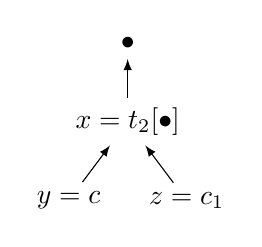
\begin{tikzpicture}[ 
  edge from parent path={(\tikzchildnode\tikzchildanchor) edge [-latex] (\tikzparentnode\tikzparentanchor)},
  level distance=1cm
]
\node (d) {$\bullet$} child{node (a) {$x=t_2[\bullet]$} child{node (b) {$y=c$}} child{node (c)
{$z=c_1$}}};

\end{tikzpicture}
\end{center}

Now each of the environments is represented by a linked list, with the binding
of $x$ shared between them. This is an example of a \emph{shared} environment
~\cite{appel1988optimizing}. This shared, linked structure dates back to the 
first machine for evaluating expressions: Landin's SECD
machine~\cite{landin1964mechanical}.

The primary insight of the $\mathcal{CE}$ machine is that it uses shared
environments to share results between instances of a variable. See \cite{cem}
for more details.

\subsection{Big Step Semantics}

Our big step semantics resemble a hybrid between Curien's calculus of closures
and Ariola et al. call-by-need operational semantics. We use terms with deBruijn
indices and close the the lambda term under a pointer into a shared environment
structure (the Heap).  

The big step semantics can be seen in Figure~\ref{fig:bigstepcem}. The
\texttt{clu} function is a partial function that looks up a closure in the
shared environment. Here we use a direct function, but later this will be
replaced by a relation, as it will clearly take a non-constant number of
instructions to execute. Our abstraction rule is identical to the call-by-name
case, and the application rule evaluates the left hand side, then binds the
argument closure to a fresh location in the heap, which extends the environment
of the function computed on the left hand side. Then if the body with this
extended environment evaluates to a value, then the application as a whole
evaluates to a value.

We define a cactus environment machine state to be well formed if, like Ariola 
et al.'s call-by-name semantics, a closure bound in the heap is closed to the
left.  Effectively, this just means that the head closure, and all closures in
the heap are closed under the heap. One advantage to using deBruijn indices is
that when referring to a fresh heap location, we don't require freshness with
respect to a substitution term, because there is no substitution. This is in
contrast to the operational semantics of Ariola et al \cite{ariola1995call}.

\begin{figure*}
\textbf{Syntax}
\begin{align*}
\tag{Term} t &::= i \; | \; \lambda t \; | \; t \; t  \\
\tag{Variable} i &\in \mathbb{N}  \\
\tag{Closure} c &::= t [l] \\
\tag{Value} v &::= \lambda t [l] \\
\tag{Heap} \mu &::= \epsilon \; | \; \mu [ l \mapsto \rho ] \\
\tag{Environment} \rho &::= \bullet \; | \; c \cdot l \\
\tag{Location} l,f &\in \mathbb{N}  \\
\tag{State} s &::= (c, \mu)
\end{align*}
\textbf{Call-by-Name Semantics}
\begin{align*}
\tag{MVal} \inference {}{(\lambda t, \mu) \rightarrow_M (\lambda t, \mu)}
\end{align*}
\begin{align*}
\tag{MApp} \inference
{(t[l], \mu) \rightarrow_{M} (\lambda t_2[l'], \mu') \quad f \not \in \textnormal{dom}(\mu') \\ 
(t_2[f], \mu'[f \mapsto t_3[l] \cdot l']) \rightarrow_{M} (v, \mu'')}
{(t \; t_3[l], \mu) \rightarrow_{M} (v, \mu'')}  
\end{align*}
\begin{align*}
\tag{MVar} \inference 
{\mu(l, i) = l' \mapsto c \cdot l'' \quad (c, \mu) \rightarrow_M (v, \mu')}
{(i[l],\mu) \rightarrow_M (v,\mu')}
\end{align*}
\textbf{Call-by-Need Semantics}
\begin{align*}
\tag{NVal} \inference{\quad}{(\lambda t, \mu) \rightarrow_N (\lambda t, \mu)}
\end{align*}
\begin{align*}
\tag{NApp} \inference
{(t[l], \mu) \rightarrow_{N} (\lambda t_2[l'], \mu') \quad f \not \in \textnormal{dom}(\mu') \\ 
(t_2[f], \mu'[f \mapsto t_3[l] \cdot l']) \rightarrow_{N} (v, \mu'')}
{(t \; t_3[l], \mu) \rightarrow_{N} (v, \mu'')}  
\end{align*}
\begin{align*}
\tag{NVar} \inference
{\mu(l, i) = l' \mapsto c \cdot l'' \quad (c, \mu) \rightarrow_N (v, \mu')}
{(i[l],\mu) \rightarrow_N (v, \mu'(l' \mapsto v \cdot l''))}
\end{align*}
\caption{Big Step Semantics for $\mathcal{CE}$}
\label{fig:bigstepcem}
\end{figure*}

\subsection{Cost Definitions}

What do we mean when we discuss the time and space complexity for a natural
semantics? Generally, we really care about the the number of instructions that
will be executed in the compiled code, and the maximum amount of memory that
will be necessary, both in the stack and the heap. One advantage to the
simplicity of the compiler for the $\mathcal{CE}$ machine is that we can define
this cost for our natural semantics in a simple way. We do this by defining a 
cost function that operates on the step function directly. This is one of the
useful features of working in a dependently typed proof asistant: we can write
functions that compute values from proof tree. Computing values from proof
objects requires defining our big step relation in the \texttt{Type} universe
instead of the \texttt{Prop} universe, but this isn't a problem.

We define two cost functions: one that computes the time for an evaluation
relation instance, and none that computes the space. Our goal is to define these
such that we can prove that the cost is preserved down through machine code. 

\begin{lstlisting}

\end{lstlisting}
